\documentclass[oneside,11pt]{article}

% Any additional packages needed should be included after jmlr2e.
% Note that jmlr2e.sty includes epsfig, amssymb, natbib and graphicx,
% and defines many common macros, such as 'proof' and 'example'.
%
% It also sets the bibliographystyle to plainnat; for more information on
% natbib citation styles, see the natbib documentation, a copy of which
% is archived at http://www.jmlr.org/format/natbib.pdf

% \usepackage{jmlr2e}
\usepackage{url}


\usepackage{mathtools}
\usepackage{graphicx}
% \usepackage{caption}
% \usepackage{subcaption}
\usepackage{amsmath}
\usepackage{amssymb}
\usepackage{enumitem}
\usepackage{algorithm}
\usepackage{multirow}
\usepackage{vhistory}

% \renewcommand*{\theHsection}{\thesection}  % this fix "destination with the same identifier" error, so leave it

%%% Custom packages %%%

% \usepackage{cleveref}

\usepackage{bm}

% For citations
\usepackage{natbib}

% convert eps to pdf
\usepackage{epstopdf}

% provides colors
\usepackage{color}
\usepackage[colorlinks=true,citecolor=blue]{hyperref}

% provides \toprule, \midrule and \bottomrule
\usepackage{booktabs}


% mdframed creates a square frame around text
% use with \begin{mdframed} \end{mdframed}
\usepackage{mdframed}


\def\block(#1,#2)#3{\multicolumn{#2}{c}{\multirow{#1}{*}{$ #3 $}}}

\newtheorem{assumption}{Assumption}

% Definitions of handy macros can go here

% get a sharper v for disambiguity
% \DeclareSymbolFont{matha}{OML}{txmi}{m}{itb}% txfonts
% \DeclareMathSymbol{\varv}{\mathord}{matha}{118}

% trace function
\DeclareMathOperator{\tr}{tr}

\newcommand{\dataset}{{\cal D}}
\newcommand{\fracpartial}[2]{\frac{\partial #1}{\partial  #2}}

%%% Custom functions %%%

% statistical independence
\newcommand\independent{\protect\mathpalette{\protect\independenT}{\perp}}
\def\independenT#1#2{\mathrel{\rlap{$#1#2$}\mkern2mu{#1#2}}}

% \argmin
\newcommand{\argmin}{\operatornamewithlimits{arg\,min}}

% \argmax
\newcommand{\argmax}{\operatornamewithlimits{arg\,max}}

% expectation and variance \E \V
\newcommand{\E}{\mathbb{E} }
\newcommand{\Var}{\mathbb{V} }

% defined for bias \B
\newcommand{\B}{\mathcal{B} }

% \dif - upright d in integrals
\newcommand*\dif{\mathop{}\!\mathrm{d}}

% \tran for transpose
\newcommand*{\T}{^{\mkern-1.5mu\mathsf{T}}}

% \highlight - highlight text in red  % require \usepackage{color}
\newcommand{\highlight}[1]{\textcolor{red}{#1}}

% \ie = i.e., \eg = e.g.,
\newcommand{\ie}{\textit{i.e.}, }
\newcommand{\eg}{\textit{e.g.}, }

% indicator symbol
\newcommand{\ind}{\bm{1}}

% \qed - end of proof
\newcommand{\qed}{\hfill {\scriptsize $\blacksquare$}}



\begin{document}

\title{IBM Data Science Capstone Project: Analysis of Singapore's Premium Product Shop Placement}

\author{Kar Wai Lim}

\maketitle


\renewcommand{\abstractname}{Executive Summary}
\begin{abstract}%   <- trailing '%' for backward compatibility of .sty file
\noindent
\begin{enumerate}
\item 
  More than 70\% of Singapore residents purchase premium 
  products in store rather than online.

\item
  Using condomium rental data in Singapore, I find out 
  the areas where Singapore residents are paying more 
  for housing rental.

\item
  I use foursquare API to look for potential 
  competitors in premium products.

\item
  Clustering algorithm is used to cluster 174,780 rental
  data into 100 groups based on location and rental per room.

\item
  Illustration using folium package allows us to determine
  the best location --- where there are many rich residents
  but little competitors.

\end{enumerate}
\end{abstract}


\section{Introduction}

Despite its small size, Singapore is one of the richest country
in the world with more than 180,000 millionaires residing in
the little red dot.\footnote{\href{https://www.straitstimes.com/business/economy/number-of-millionaires-in-singapore-up-11-to-183737-in-year-to-mid-2018-credit}{https://www.straitstimes.com/business/economy/number-of-millionaires-in-singapore-up-11-to-183737-in-year-to-mid-2018-credit}}
Interestingly, a market survey by The Nielsen Company shows that
more than 70\% of Singapore residents are purchasing premium products 
from local store rather than online.\footnote{\href{https://www.nielsen.com/sg/en/insights/article/2019/popularity-of-the-premium/}{https://www.nielsen.com/sg/en/insights/article/2019/popularity-of-the-premium/}}
This provides a great opportunity for businesses to set up 
physical premium stores in Singapore.

In this report, I will leverage the foursquare API to look for 
existing premium stores in Singapore and use condominium rental data
to determine potential areas for new businesses to set up their premium 
stores. This report will be of interest to premium stores retailer such
as Hermes and Louis Vuitton.


\section{Data}

I will be using two kinds of data in this report:
\begin{enumerate}
\item
  Foursquare location data
\item
  Condominium rental data from Urban Redevelopment Authority (URA)\footnote{\href{https://www.ura.gov.sg}{https://www.ura.gov.sg}}
\end{enumerate}


\subsection{Foursquare location data}

In particular, I will only use the venues data from Foursquare, 
which is obtainable simply by using API calls to Foursquare. While the 
details can be found in the accompanying jupyter notebook,\footnote{\href{https://github.com/karwailim/Coursera_Capstone/blob/master/Capstone_Project.ipynb}{https://github.com/karwailim/Courser\_Capstone/blob/master/Capstone\_Project.ipynb}}
I briefly describe the querying procedure.

Note that Foursquare limits the number of results returned from each API calls to 50, which is not enough to cover the whole Singapore. Thus, I use a grid based approach to split Singapore into 49 (7 X 7) regions and run an API call to each 
region (different latitude and longitude). After removing the duplicates, I obtain a total of 239 premium stores, some of these are located in Malaysia and Indonesia due to the use of large query radius. I left them in the dataset as it does not affect our analysis.

For simplicity, I use only the keywords `Premium' and `Luxury', though a more in depth studies would cover the major premium retailers in Singapore. More effort would be required in the additional steps of cleaning the data.

\subsection{Condominium rental data}

I queried the condominium data from the URA website to obtain the monthly rental associated with condominium units rented out for the past few years. The data consists of condominium name, street address, number of bedrooms, rental amount, lease date, and area. Additionally, I computed an additional row corresponding to the rental amount per number of bedrooms, as I believe this is a strong indicator to the willingness to purchase premium products (we need more data to verify this, but for the purpose of the course, we will assume this is the case).

I use Google map API to gather the condominiums latitude and longitude. Further cleaning is performed to remove the data that falls outside of Singapore (due to similar street address, missing data from Google map API, etc). After cleaning, we have a total of 174,780 rental data.


\section{Methodology}

I will keep this section brief, more details are in the notebook.

Explaratory analysis is performed to analyse the rental data, \eg
looking at the basic summary using the \texttt{.describe()} function.
Here, we can see if the data itself is appropriate, for instance, 
it is from this step I found that some of the latitude and longitude 
are incorrect (the location is in South Africa), I can then discard 
the inaccurate information as they would interfere with the analysis.

Due to the large amount of the rental data (174,780 data points), 
it is not practical to 
plot and analyse all the data using folium. Thus I use K-means, a
simple and easy to use clustering algorithm to group the data into
100 clusters that located close to one another and have a similar 
profile of rental per bedrooms. The features used in clustering are 
latitude, longitude and rental per bedrooms. Note that the features
are normalised since the numerical value for rental per bedrooms
is way larger, which would dominate the distance measure in K-means.

\section{Results and Discussions}

Using the package folium, I display the clusters with average rental 
per bedrooms greater than \$1681.67 (the median) in the map below.
The red circles correspond to regions where residents are more willing to 
pay for rental, and thus would be our business target for premium
products. We can see that the majority of the red circles are located
close to the Downtown area of Singapore (mid-bottom of the country).
This is expected as Downtown is the CBD and Financial hub of Singapore.
Again, the details are in the notebook.

Additionally, the premium stores data from Foursquare are displayed 
in little blue dots. Manually clicking the blue dots on the map allows
us to investigate the store name. Here, we observe that many premium
stores concentrate in the Downtown area as expected, 
as well as in the Changi airport (the East part of Singapore)
even though there are no rich residents. 
This is reasonable as the target audience for those stores would be
tourists from other countries.

% \begin{figure}[h!]
%     % \vskip -0.1in
    \begin{center}
        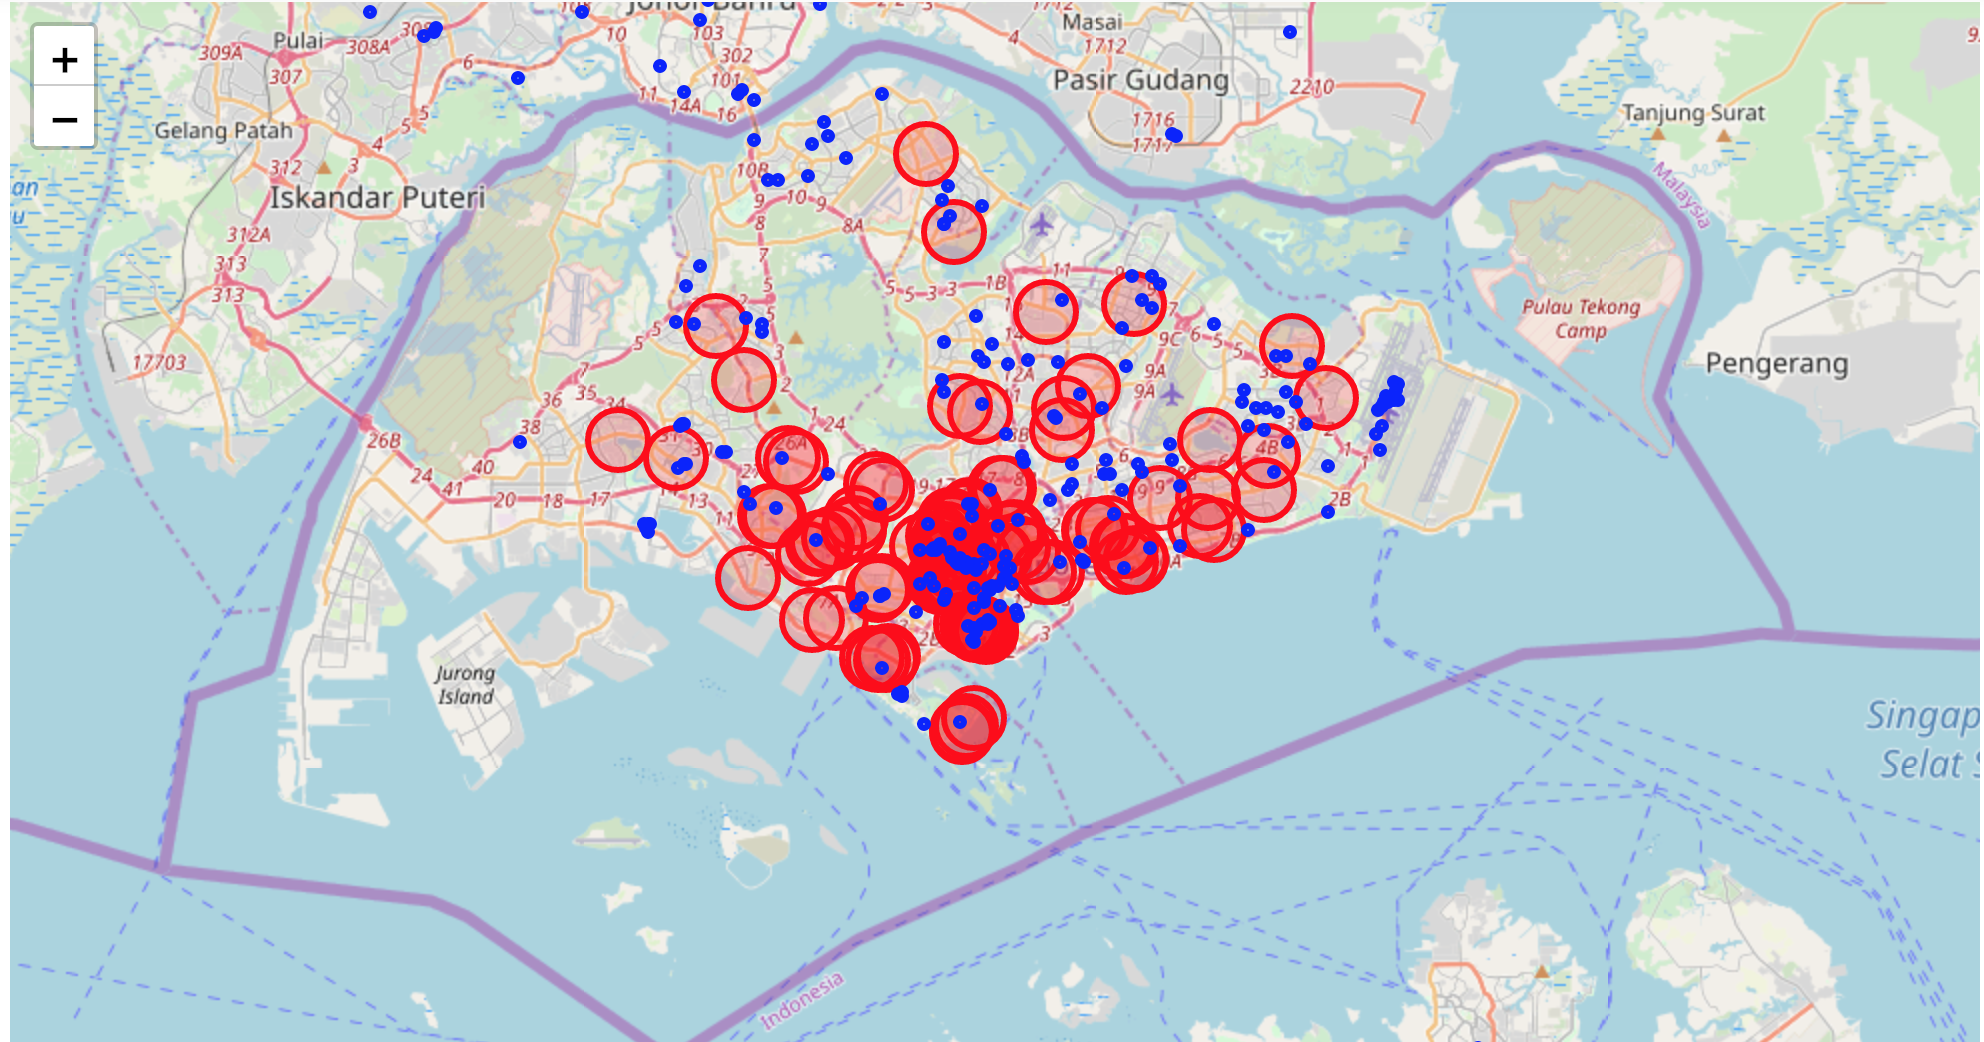
\includegraphics[width=0.96\columnwidth]{../Capstone_Project.png}
    \end{center}
%     \vskip -0.2in
% \end{figure} 

\section{Recommendations}

From the map above, we can see that there are areas in which 
rental per bedrooms are high, but not many premium stores 
are located nearby. Zooming in the map, we can see that these
areas are Lakeside, Dairy Farm, Canberra, etc. These areas 
tend to be housing areas, which I believe is the reason 
why there is no premium stores there. However, from the data,
we can see that the residents there are willing to spend 
on housing rents and thus they are good targets for premium 
products.

My recommendation is for businesses to set up their premium 
stores in these areas --- Lakeside, Dairy Farm, and Canberra.
However, I would like to note that my advice did not consider
the specific nature of the premium products (\eg luxury watches)
and might not be appropriate to all premium products. Ideally,
I would investigate in-depth the specific premium stores located
in the surrounding area and look for what is missing.

\section{Conclusion}

Many kinds of data is available out there, some readily available
and some requires additional gathering process. It is important 
for businesses to leverage these data to make an inform decision,
while supported by business experience.

In this report, we have leveraged the data from Foursquare and URA
to determine a suitable location for businesses to set up premium stores.
This is by investigating the willingness of residents to pay 
for housing rental and identifying a gap in the existing premium stores
in the areas. The best locations are found to be the areas where residents 
are paying high rental but with little presence of the existing premium stores.
In the map, these correspond to the red regions that are far away from the
blue dots.


\section*{Disclaimer}

The analysis is performed for the course on Coursera: ``Applied Data Science Capstone by IBM.'' By no means the analysis is appropriate for real 
businesses. The author Kar Wai Lim is not responsible for any loss incurred
for using the findings from this report.



\end{document}
